\chapter{Conjugacy classes of CFC elements in Coxeter groups of type $A_n$}

    In this chapter, we focus exclusively on Coxeter systems of type $A_n$.

\section{Chunks and rings}\label{sec:chunks}
    In order to formalize the ``sliding" of cylindrical heaps as first mentioned in Example~\ref{ex:A4boxes}, we develop the notion of chunks and rings.    
    Recall from Section~\ref{sec:CFC} that the CFC elements in Coxeter groups of type $A_n$ are those elements that correspond to subexpressions of Coxeter elements.
    
\begin{definition} Let $w \in \CFC(A_n)$. Then we refer to a \emph{diagonal heap (or diagonal subheap) of size $m$} as shown in Figure~\ref{fig:diagonalheap} where $k'=k+m-1$, $1 \leq k \leq n$, and $1 \leq m \leq n-k+1$.
\begin{center} \begin{figure}[H] \centering
\begin{tikzpicture}
    \sq{0}{2};    \node at (0.5,1.5)   {\scalebox{0.8}{$k$}};
    \sq{0.5}{1};  \node at (1,0.5)     {\scalebox{0.8}{$k+1$}};
                  \node at (1.5,-0.35) {$\ddots$};
    \sq{1.5}{-1}; \node at (2,-1.5)    {\scalebox{0.8}{$k'$}};
\end{tikzpicture} \caption{A diagonal heap.}\label{fig:diagonalheap}
\end{figure} \end{center}
\end{definition}

\begin{definition} Let $w \in \CFC(A_n)$. We call a convex subheap of the heap of $w$ consisting of $m$ blocks a \emph{chunk of size $m$} if it corresponds to a maximal connected component of the underlying Hasse diagram for the heap of $w$.
\end{definition}

    Notice that diagonal heaps are examples of heaps consisting of exactly one chunk.
    
\begin{example}\label{ex:chunks} Let $w \in W(A_6)$ have reduced expression $\w = 12356$. Then $w$ is CFC, and its heap is shown in Figure~\ref{fig:chunkex1}. The underlying Hasse diagram is shown in Figure~\ref{fig:chunkex2}.
    Note that there are two connected components of the Hasse diagram, and hence two chunks in $H(w)$.
    We can see the chunks in the original heap, as well. The vertical line in Figure~\ref{fig:chunkex1} shows the separation of the two chunks. The \textcolor{magenta}{pink} and \textcolor{blue}{blue} chunks can move independently in the vertical direction.

\begin{center} \begin{figure}[H] \centering
\begin{tabular}[b]{cc}
\begin{subfigure}{0.3\textwidth} \centering
\begin{tikzpicture}
    \sqm{0}{3};    \node at (0.5,2.5) {\footnotesize $1$};
    \sqm{0.5}{2};  \node at (1,1.5)   {\footnotesize $2$};
    \sqm{1}{1};    \node at (1.5,0.5) {\footnotesize $3$};
    \sqbl{2}{1};   \node at (2.5,0.5) {\footnotesize $5$};
    \sqbl{2.5}{0}; \node at (3,-0.5)  {\footnotesize $6$};
    \draw[dashed] (2,-1)--(2,3.5);
\end{tikzpicture}
\caption{}\label{fig:chunkex1}
\end{subfigure} &
\begin{subfigure}{0.3\textwidth} \centering \vspace{60pt}
\begin{tikzpicture}
\draw (0.5,2)--(1,1)--(1.5,0); \draw (2.5,1)--(3,0);
\begin{scriptsize}
    \draw [fill=black] (0.5,2) circle (1.5pt);
    \draw (0.7,2.2) node {1};
    \draw [fill=black] (1,1) circle (1.5pt);
    \draw (1.2,1.2) node {2};
    \draw [fill=black] (1.5,0) circle (1.5pt);
    \draw (1.7,0.2) node {3};
    \draw [fill=black] (2.5,1) circle (1.5pt);
    \draw (2.7,1.2) node {5};
    \draw [fill=black] (3,0) circle (1.5pt);
    \draw (3.2,0.2) node {6};
\end{scriptsize}
\end{tikzpicture}
\caption{}\label{fig:chunkex2}
\end{subfigure} \\ & \end{tabular}
\caption{The heap for a CFC element with its chunks colored \textcolor{magenta}{pink} and \textcolor{blue}{blue} together with its underlying Hasse diagram.}\label{fig:chunkex}
\end{figure} \end{center}
\end{example}

    Suppose $w,w' \in \CFC(A_n)$ such that $\hat{H}(w) = \hat{H}(w')$. Suppose $H(w)$ consists of a single chunk of size $k$. Then $H(w')$ also consists of a single chunk of size $k$ having the same blocks as $H(w)$, by Theorem~\ref{thm:e2}.
    
    Now, suppose $w,w' \in \CFC(A_n)$ such that $H(w)$ and $H(w')$ each have chunks $C$ and $C'$, respectively, with exactly the same blocks but not necessarily in the same configuration. Then it follows from Theorem~\ref{thm:e2} that we can obtain $C'$ by applying cyclic shifts to $C$.
    In this case, we say that $C$ and $C'$ are \emph{chunk equivalent}.
    Observe that two chunks are chunk equivalent if and only if they differ by a sequence of cyclic shifts. This generates an equivalence relation on the set of possible chunks of heaps for CFC elements in $W(A_n)$.

    Define $\hat{C}$ to be the equivalence class of the chunk $C$, which we visualize by wrapping representatives on a cylinder. It is easy to show that every chunk equivalence class contains a diagonal representative.
    We call the equivalence class of a chunk a \emph{ring}. That is, a ring is a chunk wrapped on a cylinder.
    
    For each $w \in \CFC(A_n)$, $\hat{H}(w)$ can be thought of as a disjoint union of rings. We can obtain a new cylindrical heap by \emph{sliding} rings by adding some $j \in \Z$ to the label of each block in the ring.
    We say two rings are \emph{slide equivalent} if we can slide one ring $j \in \Z$ spaces to obtain the other ring.
    Note that two rings that are slide equivalent have the same number of blocks.
    Two cylindrical heaps are \emph{slide equivalent} if we can slide the rings of one cylindrical heap to obtain the other cylindrical heap.
    Note that the corresponding rings are in the same order.

\begin{example} Let $w,y \in \CFC(A_9)$ have reduced expressions $\w = 124567$ and $\y = 236789$, respectively.
    Then the cylindrical heaps corresponding to $H(w)$ and $H(y)$ are shown in Figure~\ref{fig:slideexample1.1} and~\ref{fig:slideexample1.2}, respectively. Each of the cylindrical heaps consists of two rings.
    We can see that $\hat{H}(w)$ and $\hat{H}(y)$ are slide equivalent since we can add one to each of the labels of the blocks in the first ring of $\hat{H}(w)$ to obtain the first ring of $\hat{H}(y)$ and add two to each of the blocks in the second ring of $\hat{H}(w)$ to obtain the second ring of $\hat{H}(y)$.
\begin{center} \begin{figure}[H] \centering
\begin{subfigure}{0.4\textwidth} \centering
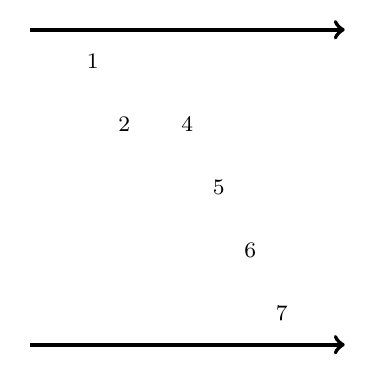
\begin{tikzpicture}[scale=0.8]
\draw[line width=1.5pt,->] (-0.5,3)--(4.5,3);
    \sq{0}{3};   \node at (0.5,2.5) {\footnotesize $1$};
    \sq{0.5}{2}; \node at (1,1.5)   {\footnotesize $2$};
    \sq{1.5}{2}; \node at (2,1.5)   {\footnotesize $4$};
    \sq{2}{1};   \node at (2.5,0.5) {\footnotesize $5$};
    \sq{2.5}{0}; \node at (3,-0.5)  {\footnotesize $6$};
    \sq{3}{-1};  \node at (3.5,-1.5){\footnotesize $7$};
\draw[line width=1.5pt,->] (-0.5,-2)--(4.5,-2);
\end{tikzpicture}
\caption{}\label{fig:slideexample1.1}
\end{subfigure}
\begin{subfigure}{0.4\textwidth} \centering
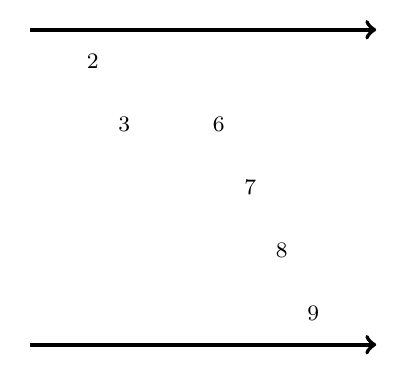
\begin{tikzpicture}[scale=0.8]
\draw[line width=1.5pt,->] (-0.5,3)--(5,3);
    \sq{0}{3};   \node at (0.5,2.5) {\footnotesize $2$};
    \sq{0.5}{2}; \node at (1,1.5)   {\footnotesize $3$};
    \sq{2}{2};   \node at (2.5,1.5) {\footnotesize $6$};
    \sq{2.5}{1}; \node at (3,0.5)   {\footnotesize $7$};
    \sq{3}{0};   \node at (3.5,-0.5){\footnotesize $8$};
    \sq{3.5}{-1};\node at (4,-1.5)  {\footnotesize $9$};
\draw[line width=1.5pt,->] (-0.5,-2)--(5,-2);
\end{tikzpicture}
\caption{}\label{fig:slideexample1.2}
\end{subfigure}
\caption{Two slide equivalent cylindrical heaps.}\label{}
\end{figure} \end{center}
\end{example}
    
\begin{definition}
Suppose $w,w' \in \CFC(A_n)$ are such that $\hat{H}(w)$ and $\hat{H}(w')$ consist exactly of the rings $R_1,\ldots,R_k$ and $R_1',\ldots,R_k'$, respectively.
    Then $\hat{H}(w)$ and $\hat{H}(w')$ are \emph{ring equivalent} if there exists a bijection $R_i \longleftrightarrow R_i'$ such that $R_i$ and $R_i'$ consist of the same number of blocks (not necessarily with the same labels).
\end{definition}
    
\begin{example} Let $w \in W(A_6)$ have reduced expression $\w = 12356$. Then $w$ is CFC, and its heap is shown in Figure~\ref{fig:chunkex1}. Recall that the heap consists of two chunks.
    The cylindrical heap $\hat{H}(w)$ is shown in Figure~\ref{fig:cylheapex1} and the rings are the chunks wrapped on a cylinder, i.e., the rings are as shown in Figure~\ref{fig:cylheapex2}.
    We see that the cylindrical heap in Figure~\ref{fig:cylheapex3} is ring equivalent to $\hat{H}(w)$ because there are exactly two rings, one of size three and one of size two, in each cylindrical heap.

\begin{center} \begin{figure}[H] \centering
\begin{subfigure}{0.4\textwidth} \centering
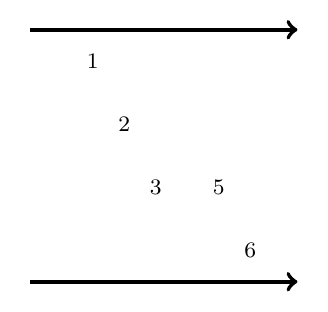
\begin{tikzpicture}[scale=0.8]
\draw[line width=1.5pt,->] (-0.5,3)--(3.75,3);
    \sq{0}{3};   \node at (0.5,2.5) {\footnotesize $1$};
    \sq{0.5}{2}; \node at (1,1.5)   {\footnotesize $2$};
    \sq{1}{1};   \node at (1.5,0.5) {\footnotesize $3$};
    \sq{2}{1};   \node at (2.5,0.5) {\footnotesize $5$};
    \sq{2.5}{0}; \node at (3,-0.5)  {\footnotesize $6$};
\draw[line width=1.5pt,->] (-0.5,-1)--(3.75,-1);
\end{tikzpicture}
\caption{}\label{fig:cylheapex1}
\end{subfigure}
\begin{subfigure}{0.4\textwidth} \centering \vspace{20pt}
\begin{tabular}{ccc}
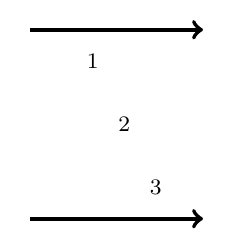
\begin{tikzpicture}[scale=0.8]
\draw[line width=1.5pt,->] (-0.5,3)--(2.25,3); \draw[line width=1.5pt,->] (-0.5,0)--(2.25,0);
    \sq{0}{3};   \node at (0.5,2.5) {\footnotesize $1$};
    \sq{0.5}{2}; \node at (1,1.5)   {\footnotesize $2$};
    \sq{1}{1};   \node at (1.5,0.5) {\footnotesize $3$};
\end{tikzpicture} &&
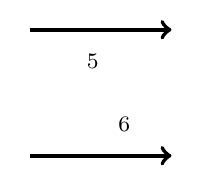
\begin{tikzpicture}[scale=0.8]
\draw[line width=1.5pt,->] (-0.5,1)--(1.75,1); \draw[line width=1.5pt,->] (-0.5,-1)--(1.75,-1);
    \sq{0}{1};   \node at (0.5,0.5) {\footnotesize $5$};
    \sq{0.5}{0}; \node at (1,-0.5)  {\footnotesize $6$};
\end{tikzpicture} \end{tabular}
\caption{}\label{fig:cylheapex2}
\end{subfigure}
\caption{The cylindrical heap and rings for some CFC element.\label{fig:cylheap}}
\end{figure} \end{center}

\begin{figure}[H] \centering \vspace{-30pt}
\begin{subfigure}{0.4\textwidth} \centering
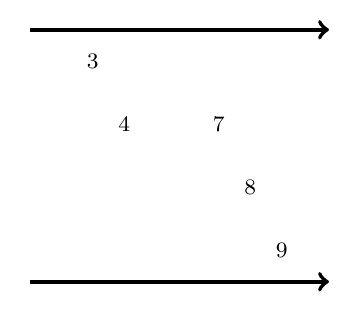
\begin{tikzpicture}[scale=0.8]
\draw[line width=1.5pt,->] (-0.5,3)--(4.25,3);
    \sq{0}{3};   \node at (0.5,2.5) {\footnotesize $3$};
    \sq{0.5}{2}; \node at (1,1.5)   {\footnotesize $4$};
    \sq{2}{2};   \node at (2.5,1.5) {\footnotesize $7$};
    \sq{2.5}{1}; \node at (3,0.5)   {\footnotesize $8$};
    \sq{3}{0};   \node at (3.5,-0.5){\footnotesize $9$};
\draw[line width=1.5pt,->] (-0.5,-1)--(4.25,-1);
\end{tikzpicture}
\caption{}\label{cylheapex3.1}
\end{subfigure}
\begin{subfigure}{0.4\textwidth} \centering \vspace{18pt}
\begin{tabular}{ccc}
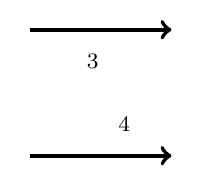
\begin{tikzpicture}[scale=0.8]
\draw[line width=1.5pt,->] (-0.5,1)--(1.75,1); \draw[line width=1.5pt,->] (-0.5,-1)--(1.75,-1);
    \sq{0}{1};   \node at (0.5,0.5) {\footnotesize $3$};
    \sq{0.5}{0}; \node at (1,-0.5)  {\footnotesize $4$};
\end{tikzpicture} &&
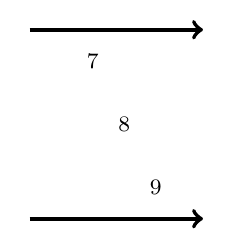
\begin{tikzpicture}[scale=0.8]
\draw[line width=1.5pt,->] (-0.5,3)--(2.25,3); \draw[line width=1.5pt,->] (-0.5,0)--(2.25,0);
    \sq{0}{3};   \node at (0.5,2.5) {\footnotesize $7$};
    \sq{0.5}{2}; \node at (1,1.5)   {\footnotesize $8$};
    \sq{1}{1};   \node at (1.5,0.5) {\footnotesize $9$};
\end{tikzpicture} \end{tabular}
\caption{}\label{fig:cylheapex3.2}
\end{subfigure}
\caption{A cylindrical heap ring equivalent to the one in Figure~\ref{fig:cylheapex1} together with its rings.}\label{fig:cylheapex3}
\end{figure}
\end{example}

\begin{definition}
We refer to a heap as \emph{simple} if it is as shown in Figure~\ref{fig:simple}, where each chunk is diagonal, the leftmost chunk starts at 1, and the chunks are as close to each other as possible.
\begin{center} \begin{figure}[H] \centering
\begin{tabular}{m{2cm} m{2cm} m{2cm} m{0.5cm} m{2cm}}
\begin{tikzpicture}[scale=0.95]
    \sq{0}{3};    \node at (0.5,2.5) {\scalebox{0.8}{$1$}};
    \sq{0.5}{2};  \node at (1,1.5)   {\scalebox{0.8}{$2$}};
                  \node at (1.5,0.7) {$\ddots$};
    \sq{1.5}{0};  \node at (2,-0.5)  {\scalebox{0.8}{$k$}};
\end{tikzpicture} &
\begin{tikzpicture}[scale=0.95]
    \sq{2.5}{3};  \node at (3,2.5)   {\scalebox{0.8}{$k+2$}};
    \sq{3}{2};    \node at (3.5,1.5) {\scalebox{0.8}{$k+3$}};
                  \node at (4,0.7)   {$\ddots$};
    \sq{4}{0};    \node at (4.5,-0.5){\scalebox{0.8}{$k'$}};
\end{tikzpicture} &
\begin{tikzpicture}[scale=0.95]
    \sq{2.5}{3};  \node at (3,2.5)   {\scalebox{0.8}{$k'+2$}};
    \sq{3}{2};    \node at (3.5,1.5) {\scalebox{0.8}{$k'+3$}};
                  \node at (4,0.7)   {$\ddots$};
    \sq{4}{0};    \node at (4.5,-0.5){\scalebox{0.8}{$k''$}};
\end{tikzpicture} & $\cdots$ &
\begin{tikzpicture}[scale=0.95]
    \sq{2.5}{3};  \node at (3,2.5)   {\scalebox{0.8}{$h+2$}};
    \sq{3}{2};    \node at (3.5,1.5) {\scalebox{0.8}{$h+3$}};
                  \node at (4,0.7)   {$\ddots$};
    \sq{4}{0};    \node at (4.5,-0.5){\scalebox{0.8}{$h'$}};
\end{tikzpicture}
\end{tabular}
\caption{A simple heap.}\label{fig:simple}
\end{figure}
\end{center}
\end{definition}

\begin{remark} Note that if $w \in \CFC(A_n)$, then there exists some $y \in \CFC(A_n)$ having a simple heap such that $\hat{H}(w)$ is ring equivalent to $\hat{H}(y)$.
\end{remark}

\section{Conjugacy classes of CFC elements in $W(A_n)$}\label{sec:conjugacyofCFC}
    In this section, we give a constructive description of conjugate CFC elements. The goal of this section is to prove the following theorem.
    
\begin{theorem}\label{thm:conjiffring} Let $w,y \in \CFC(A_n)$. Then $w$ and $y$ are conjugate if and only if $\hat{H}(w)$ and $\hat{H}(y)$ are ring equivalent.
\end{theorem}

    The following example motivates the proof of Lemma~\ref{lem:slide}.

\begin{example}\label{ex:slide} Let $w,y \in W(A_7)$ have reduced expressions $\w = 3456$ and $\y = 4567$, respectively. Note that $w$ and $y$ are both CFC, so there is a unique heap for each, as shown in Figures~\ref{fig:slideex0.1} and~\ref{fig:slideex0.2}, respectively. Notice that $\hat{H}(w)$ and $\hat{H}(y)$ are ring equivalent.

\begin{center} \begin{figure}[H] \centering
\begin{subfigure}{0.3\textwidth} \centering
\begin{tikzpicture}[scale=0.85]
    \sq{0}{10};       \node at (0.5,9.5) {\footnotesize $3$};
    \sq{0.5}{9};      \node at (1,8.5)   {\footnotesize $4$};
    \sq{1}{8};        \node at (1.5,7.5) {\footnotesize $5$};
    \sq{1.5}{7};      \node at (2,6.5)   {\footnotesize $6$};
\end{tikzpicture}
\caption{}\label{fig:slideex0.1}
\end{subfigure}
\begin{subfigure}{0.3\textwidth} \centering
\begin{tikzpicture}[scale=0.85]
    \sq{0}{10};       \node at (0.5,9.5) {\footnotesize $4$};
    \sq{0.5}{9};      \node at (1,8.5)   {\footnotesize $5$};
    \sq{1}{8};        \node at (1.5,7.5) {\footnotesize $6$};
    \sq{1.5}{7};      \node at (2,6.5)   {\footnotesize $7$};
\end{tikzpicture}
\caption{}\label{fig:slideex0.2}
\end{subfigure}
\caption{The heaps for Example~\ref{ex:slide}.}\label{fig:slideex0}
\end{figure} \end{center}

    We claim that we can obtain $y$ by conjugating $w$ by $x$, where $x$ has reduced expression $\x = 34567$.
    Then the heap of ${\x}{\w}{\x^{-1}}$ is shown in Figure~\ref{fig:slideexheap1}, where the \textcolor{orange}{orange} blocks correspond to the heap of $x$, the \textcolor{blue}{blue} blocks correspond to the heap of $w$, and the \textcolor{ggreen}{green} blocks correspond to the heap of $x^{-1}$.
    Then applying Lemma~\ref{lem:stst} to the extra long $76$-chain, denoted in the heap in Figure~\ref{fig:slideexheap1} by the hatched blocks, we get the heap shown in Figure~\ref{fig:slideexheap2}.
    Now we can apply Lemma~\ref{lem:stst} to the extra long $65$-chain to get the heap in Figure~\ref{fig:slideexheap3}.
    Continuing in this manner, applying Lemma~\ref{lem:stst} to the new extra long $s_is_j$-chains created, we get the heap in Figure~\ref{fig:slideexheap4.1}.
    Applying Lemma~\ref{lem:stst} to the extra long $34$-chain, denoted in the heap by the hatched blocks, we get the heap in Figure~\ref{fig:slideexheap4.2}.
    Then, canceling the two adjacent $3$ blocks, denoted in the heap by the checked blocks, the result follows, as shown in Figure~\ref{fig:slideexheap4.3}.
    
\begin{center} \begin{figure}[H] \centering
\begin{subfigure}{0.3\textwidth} \centering
\begin{tikzpicture}
    \sqor{0}{10};       \node at (0.5,9.5) {\footnotesize $3$};
    \sqor{0.5}{9};      \node at (1,8.5)   {\footnotesize $4$};
    \sqor{1}{8};        \node at (1.5,7.5) {\footnotesize $5$};
    \sqor{1.5}{7};      \node at (2,6.5)   {\footnotesize $6$};
    \sqorhash{2}{6};    \node at (2.5,5.5) {\footnotesize $7$};
    \sqbl{0}{8};        \node at (0.5,7.5) {\footnotesize $3$};
    \sqbl{0.5}{7};      \node at (1,6.5)   {\footnotesize $4$};
    \sqbl{1}{6};        \node at (1.5,5.5) {\footnotesize $5$};
    \sqblhash{1.5}{5};  \node at (2,4.5)   {\footnotesize $6$};
    \sqgrhash{2}{4};    \node at (2.5,3.5) {\footnotesize $7$};
    \sqgrhash{1.5}{3};  \node at (2,2.5)   {\footnotesize $6$};
    \sqgr{1}{2};        \node at (1.5,1.5) {\footnotesize $5$};
    \sqgr{0.5}{1};      \node at (1,0.5)   {\footnotesize $4$};
    \sqgr{0}{0};        \node at (0.5,-0.5){\footnotesize $3$};
\end{tikzpicture}
\caption{}\label{fig:slideexheap1}
\end{subfigure}
\begin{subfigure}{0.3\textwidth} \centering \vspace{56pt}
\begin{tikzpicture}
    \sqor{0}{10};       \node at (0.5,9.5) {\footnotesize $3$};
    \sqor{0.5}{9};      \node at (1,8.5)   {\footnotesize $4$};
    \sqor{1}{8};        \node at (1.5,7.5) {\footnotesize $5$};
    \sqorhash{1.5}{7};  \node at (2,6.5)   {\footnotesize $6$};
    \sqbl{0}{8};        \node at (0.5,7.5) {\footnotesize $3$};
    \sqbl{0.5}{7};      \node at (1,6.5)   {\footnotesize $4$};
    \sqblhash{1}{6};    \node at (1.5,5.5) {\footnotesize $5$};
    \sqblhash{1.5}{5};  \node at (2,4.5)   {\footnotesize $6$};
    \sqgr{2}{4};        \node at (2.5,3.5) {\footnotesize $7$};
    \sqgrhash{1}{4};    \node at (1.5,3.5) {\footnotesize $5$};
    \sqgr{0.5}{3};      \node at (1,2.5)   {\footnotesize $4$};
    \sqgr{0}{2};        \node at (0.5,1.5) {\footnotesize $3$};
\end{tikzpicture}
\caption{}\label{fig:slideexheap2}
\end{subfigure}
\begin{subfigure}{0.3\textwidth} \centering \vspace{112pt}
\begin{tikzpicture}
    \sqor{0}{10};       \node at (0.5,9.5) {\footnotesize $3$};
    \sqor{0.5}{9};      \node at (1,8.5)   {\footnotesize $4$};
    \sqorhash{1}{8};    \node at (1.5,7.5) {\footnotesize $5$};
    \sqbl{0}{8};        \node at (0.5,7.5) {\footnotesize $3$};
    \sqblhash{0.5}{7};  \node at (1,6.5)   {\footnotesize $4$};
    \sqblhash{1}{6};    \node at (1.5,5.5) {\footnotesize $5$};
    \sqbl{1.5}{5};      \node at (2,4.5)   {\footnotesize $6$};
    \sqgr{2}{4};        \node at (2.5,3.5) {\footnotesize $7$};
    \sqgrhash{0.5}{5};  \node at (1,4.5)   {\footnotesize $4$};
    \sqgr{0}{4};        \node at (0.5,3.5) {\footnotesize $3$};
\end{tikzpicture}
\caption{}\label{fig:slideexheap3}
\end{subfigure}
\caption{The heaps for Example~\ref{ex:slide}.}\label{}
\end{figure} \end{center}
\begin{figure}[H] \centering
\ContinuedFloat
\begin{subfigure}{0.3\textwidth} \centering
\begin{tikzpicture}
    \sqorhash{0}{10};   \node at (0.5,9.5) {\footnotesize $3$};
    \sqorhash{0.5}{9};  \node at (1,8.5)   {\footnotesize $4$};
    \sqblhash{0}{8};    \node at (0.5,7.5) {\footnotesize $3$};
    \sqblhash{0.5}{7};  \node at (1,6.5)   {\footnotesize $4$};
    \sqbl{1}{6};        \node at (1.5,5.5) {\footnotesize $5$};
    \sqbl{1.5}{5};      \node at (2,4.5)   {\footnotesize $6$};
    \sqgr{2}{4};        \node at (2.5,3.5) {\footnotesize $7$};
    \sqgr{0}{6};        \node at (0.5,5.5) {\footnotesize $3$};
\end{tikzpicture}
\caption{}\label{fig:slideexheap4.1}
\end{subfigure}
\begin{subfigure}{0.3\textwidth} \centering \vspace{55pt}
\begin{tikzpicture}
    \sqor{0.5}{8};      \node at (1,7.5)   {\footnotesize $4$};
    \sqblcheck{0}{7};   \node at (0.5,6.5) {\footnotesize $3$};
    \sqbl{1}{6};        \node at (1.5,5.5) {\footnotesize $5$};
    \sqbl{1.5}{5};      \node at (2,4.5)   {\footnotesize $6$};
    \sqgr{2}{4};        \node at (2.5,3.5) {\footnotesize $7$};
    \sqgrcheck{0}{6};   \node at (0.5,5.5) {\footnotesize $3$};
\end{tikzpicture}
\caption{}\label{fig:slideexheap4.2}
\end{subfigure}
\begin{subfigure}{0.3\textwidth} \centering \vspace{80pt}
\begin{tikzpicture}
    \sqbl{0.5}{7};      \node at (1,6.5)   {\footnotesize $4$};
    \sqbl{1}{6};        \node at (1.5,5.5) {\footnotesize $5$};
    \sqbl{1.5}{5};      \node at (2,4.5)   {\footnotesize $6$};
    \sqgr{2}{4};        \node at (2.5,3.5) {\footnotesize $7$};
\end{tikzpicture}
\caption{}\label{fig:slideexheap4.3}
\end{subfigure}
\caption{The heaps for Example~\ref{ex:slide} (continued).}\label{fig:slideex}
\end{figure}
\end{example}

    We can generalize the technique used in the previous example to prove the following lemma, which shows that two CFC elements are conjugate if their cylindrical heaps are slide equivalent by one space.
    
\begin{lemma}\label{lem:slide}
Let $w \in \CFC(A_n)$. Suppose $H(w)$ has a diagonal chunk $C$ where the largest label of $C$ is $k' \leq n-1$.
    Let $y \in \CFC(A_n)$ such that $\hat{H}(y)$ is slide equivalent to $\hat{H}(w)$ by sliding $\hat{C}$, the ring for the chunk $C$, one space to the right. Then $y$ and $w$ are conjugate.
    That is, we can slide the ring in Figure~\ref{fig:slide1} to the ring in Figure~\ref{fig:slide2}, where $k' = k+m$ for some $m$ via conjugation.
\end{lemma}

\begin{center} \begin{figure}[H] \centering
\begin{subfigure}{0.3\textwidth} \centering
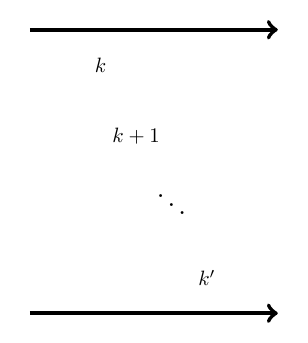
\begin{tikzpicture}[scale=0.9]
\draw[line width=1.5pt,->] (-0.5,2)--(3,2); \draw[line width=1.5pt,->] (-0.5,-2)--(3,-2);
    \sq{0}{2};    \node at (0.5,1.5)   {\scalebox{0.75}{$k$}};
    \sq{0.5}{1};  \node at (1,0.5)     {\scalebox{0.75}{$k+1$}};
                  \node at (1.5,-0.35) {$\ddots$};
    \sq{1.5}{-1}; \node at (2,-1.5)    {\scalebox{0.75}{$k'$}};
\end{tikzpicture}
\caption{}\label{fig:slide1}
\end{subfigure}
\begin{subfigure}{0.3\textwidth} \centering
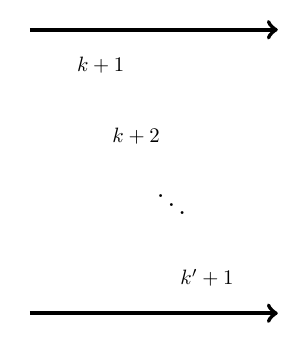
\begin{tikzpicture}[scale=0.9]
\draw[line width=1.5pt,->] (-0.5,2)--(3,2); \draw[line width=1.5pt,->] (-0.5,-2)--(3,-2);
    \sq{0}{2};    \node at (0.5,1.5)   {\scalebox{0.75}{$k+1$}};
    \sq{0.5}{1};  \node at (1,0.5)     {\scalebox{0.75}{$k+2$}};
                  \node at (1.5,-0.35) {$\ddots$};
    \sq{1.5}{-1}; \node at (2,-1.5)    {\scalebox{0.75}{$k'+1$}};
\end{tikzpicture}
\caption{}\label{fig:slide2}
\end{subfigure}
\caption{The rings for Lemma~\ref{lem:slide}.}\label{fig:slidelemma}
\end{figure} \end{center}

\begin{proof} Without loss of generality, assume $H(w)$ consists of a diagonal single chunk, where $\w = (k)(k+1) \cdots (k')$ is a reduced expression for $w$.
    Notice that this implies there is no block in $H(w)$ labeled by $k'+1$.

    Let $x$ have reduced expression $\x = (k)(k+1) \cdots (k')(k'+1)$. Then a heap of $w$ conjugated by $x$, namely, $H({\x}{\w}{\x^{-1}})$, is shown in Figure~\ref{fig:slideheap1}, where the \textcolor{orange}{orange} blocks correspond to the heap of $x$, the \textcolor{blue}{blue} blocks correspond to the heap of $w$, and the \textcolor{ggreen}{green} blocks correspond to the heap of $x^{-1}$.
    Then, we have an extra long $(k'+1)(k')$-chain, denoted in the heap by the hatched blocks.
    By Lemma~\ref{lem:stst}, we get the heap in Figure~\ref{fig:slideheap2} since the \textcolor{orange}{orange} $k'+1$ block and the \textcolor{ggreen}{green} $k'$ block are eliminated.
    Now, in the new heap in Figure~\ref{fig:slideheap2}, we have an extra long $(k')(k'-1)$-chain, denoted by the hatched blocks, so applying Lemma~\ref{lem:stst} again, we eliminate the \textcolor{orange}{orange} $k'$ block and the \textcolor{ggreen}{green} $k'-1$ block.
    
    Continuing in this manner, applying $m$ iterations of Lemma~\ref{lem:stst} to $m$ extra long $s_is_j$-chains, we get the heap shown in Figure~\ref{fig:slideheap3.1}.
    After applying Lemma~\ref{lem:stst} to the extra long $(k)(k+1)$-chain, denoted in the heap by the hatched blocks, we get the heap in Figure~\ref{fig:slideheap3.2}.
    Then, canceling the two adjacent $k$ blocks, denoted in the heap by the checked blocks, the result follows, as shown in Figure~\ref{fig:slideheap3.3}.
    Note that the last application of Lemma~\ref{lem:stst} was to an extra long $(k)(k+1)$-chain located at the top of the heap.
\end{proof}

\begin{center} \begin{figure}[htpb] \centering
\begin{subfigure}{0.3\textwidth} \centering
\begin{tikzpicture}[scale=0.9]
    \sqor{0}{12};       \node at (0.5,11.5){\scalebox{0.8}{$k$}};
    \sqor{0.5}{11};     \node at (1,10.5)  {\scalebox{0.8}{$k+1$}};
    \sqor{1}{10};       \node at (1.5,9.5) {\scalebox{0.8}{$k+2$}};
                        \node at (2.55,8.7){$\ddots$};
    \sqor{2.5}{8};      \node at (3,7.5)   {\scalebox{0.8}{$k'$}};
    \sqorhash{3}{7};    \node at (3.5,6.5) {\scalebox{0.8}{$k'+1$}};
    \sqbl{0}{10};       \node at (0.5,9.5) {\scalebox{0.8}{$k$}};
    \sqbl{0.5}{9};      \node at (1,8.5)   {\scalebox{0.8}{$k+1$}};
                        \node at (1.5,7.6) {$\ddots$};
    \sqbl{2}{7};        \node at (2.5,6.5) {\scalebox{0.8}{$k'-1$}};
    \sqblhash{2.5}{6};  \node at (3,5.5)   {\scalebox{0.8}{$k'$}};
    \sqgrhash{3}{5};    \node at (3.5,4.5) {\scalebox{0.8}{$k'+1$}};
    \sqgrhash{2.5}{4};  \node at (3,3.5)   {\scalebox{0.8}{$k'$}};
    \sqgr{2}{3};        \node at (2.5,2.5) {\scalebox{0.8}{$k'-1$}};
                        \node at (1.9,1.6) {$\iddots$};
    \sqgr{0.5}{1};      \node at (1,0.5)   {\scalebox{0.8}{$k+1$}};
    \sqgr{0}{0};        \node at (0.5,-0.5){\scalebox{0.8}{$k$}};
\end{tikzpicture}
\caption{}\label{fig:slideheap1}
\end{subfigure}
\begin{subfigure}{0.3\textwidth} \centering \vspace{49pt}
\begin{tikzpicture}[scale=0.9]
    \sqor{0}{12};   \node at (0.5,11.5){\scalebox{0.8}{$k$}};
    \sqor{0.5}{11}; \node at (1,10.5)  {\scalebox{0.8}{$k+1$}};
    \sqor{1}{10};   \node at (1.5,9.5) {\scalebox{0.8}{$k+2$}};
                    \node at (2.55,8.7){$\ddots$};
    \sqorhash{2.5}{8};\node at (3,7.5) {\scalebox{0.8}{$k'$}};
    
    \sqbl{0}{10};   \node at (0.5,9.5) {\scalebox{0.8}{$k$}};
    \sqbl{0.5}{9};  \node at (1,8.5)   {\scalebox{0.8}{$k+1$}};
                    \node at (1.5,7.6) {$\ddots$};
    \sqblhash{2}{7};\node at (2.5,6.5) {\scalebox{0.8}{$k'-1$}};
    \sqblhash{2.5}{6};\node at (3,5.5) {\scalebox{0.8}{$k'$}};
    
    \sqgr{3}{5};    \node at (3.5,4.5) {\scalebox{0.8}{$k'+1$}};
    \sqgrhash{2}{5};\node at (2.5,4.5) {\scalebox{0.8}{$k'-1$}};
                    \node at (2,3.5)   {$\iddots$};
    \sqgr{0.5}{3};  \node at (1,2.5)   {\scalebox{0.8}{$k+1$}};
    \sqgr{0}{2};    \node at (0.5,1.5) {\scalebox{0.8}{$k$}};
\end{tikzpicture}
\caption{}\label{fig:slideheap2}
\end{subfigure}
\begin{subfigure}{0.3\textwidth} \centering \vspace{102pt}
\begin{tikzpicture}
    \sqorhash{0}{7};    \node at (0.5,6.5) {\scalebox{0.8}{$k$}};
    \sqorhash{0.5}{6};  \node at (1,5.5)   {\scalebox{0.8}{$k+1$}};
    \sqgr{0}{3};        \node at (0.5,2.5) {\scalebox{0.8}{$k$}};
    \sqblhash{0}{5};    \node at (0.5,4.5) {\scalebox{0.8}{$k$}};
    \sqblhash{0.5}{4};  \node at (1,3.5)   {\scalebox{0.8}{$k+1$}};
    \sqbl{1}{3};        \node at (1.5,2.5) {\scalebox{0.8}{$k+2$}};
                        \node at (2.4,1.7) {$\ddots$};
    \sqbl{2.5}{1};      \node at (3,0.5)   {\scalebox{0.8}{$k'$}};
    \sqgr{3}{0};        \node at (3.5,-0.5){\scalebox{0.8}{$k'+1$}};
\end{tikzpicture}
\caption{}\label{fig:slideheap3.1}
\end{subfigure}
\begin{subfigure}{0.3\textwidth} \centering \vspace{20pt}
\begin{tikzpicture}
    \sqor{0.5}{5};      \node at (1,4.5)   {\scalebox{0.8}{$k+1$}};
    \sqgrcheck{0}{3};   \node at (0.5,2.5) {\scalebox{0.8}{$k$}};
    \sqblcheck{0}{4};   \node at (0.5,3.5) {\scalebox{0.8}{$k$}};
    \sqbl{1}{3};        \node at (1.5,2.5) {\scalebox{0.8}{$k+2$}};
                        \node at (2.4,1.7) {$\ddots$};
    \sqbl{2.5}{1};      \node at (3,0.5)   {\scalebox{0.8}{$k'$}};
    \sqgr{3}{0};        \node at (3.5,-0.5){\scalebox{0.8}{$k'+1$}};
\end{tikzpicture}\caption{}\label{fig:slideheap3.2}
\end{subfigure}
\begin{subfigure}{0.3\textwidth} \centering \vspace{48pt}
\begin{tikzpicture}
    \sqor{0.5}{4};      \node at (1,3.5)   {\scalebox{0.8}{$k+1$}};
    \sqbl{1}{3};        \node at (1.5,2.5) {\scalebox{0.8}{$k+2$}};
                        \node at (2.4,1.7) {$\ddots$};
    \sqbl{2.5}{1};      \node at (3,0.5)   {\scalebox{0.8}{$k'$}};
    \sqgr{3}{0};        \node at (3.5,-0.5){\scalebox{0.8}{$k'+1$}};
\end{tikzpicture}
\caption{}\label{fig:slideheap3.3}
\end{subfigure}
\caption{The heaps for Lemma~\ref{lem:slide}.}\label{fig:slideheaps}
\end{figure} \end{center}


\begin{remark}\label{rem:slide} Suppose $\hat{H}(w)$ and $\hat{H}(y)$ are slide equivalent by sliding rings of $\hat{H}(w)$ one space to the right to obtain $\hat{H}(y)$.
    Equivalently, we can obtain $\hat{H}(w)$ by sliding rings of $\hat{H}(y)$ one space to the left. In this case, we can obtain $w$ by conjugating $y$ by $x^{-1}$, where $x$ is as given in the proof of Lemma~\ref{lem:slide}.
    It follows that if $w,y \in \CFC(A_n)$ such that $\hat{H}(w)$ is slide equivalent to $\hat{H}(y)$, then $w$ is conjugate to $y$ since we can cyclically shift chunks of $H(w)$ to obtain diagonal chunks and then use Lemma~\ref{lem:slide} as necessary to shift the diagonal chunks. We can then obtain the chunks of $H(y)$ by doing the appropriate cyclic shifts.
\end{remark}

\pagebreak
    We now state a lemma that will be useful in the proof of the lemma that follows.

\begin{lemma} \label{lem:boomerang} Let $w \in W(A_n)$ have reduced expression $\w$. If $H(\w)$ has the heap shown in Figure~\ref{fig:boomerang1} as a convex subheap, then we can replace it with the convex subheap shown in Figure~\ref{fig:boomerang2} to obtain another heap for $w$.
\end{lemma}
\begin{proof} It follows from the relations in $W(A_n)$ that the subword \begin{equation} \label{eq:boom1} (k)(k+1) \cdots (k')(k'+1)(k') \cdots (k+1)(k) \end{equation} can be transformed into \begin{equation} \label{eq:boom2} (k'+1)(k') \cdots (k+1)(k)(k+1) \cdots (k')(k'+1), \end{equation} where $k'=k+m$, by performing a sequence of braid moves.
    In the heap, the subword in (\ref{eq:boom1}) corresponds to the convex subheap shown in Figure~\ref{fig:boomerang1} and the subword in (\ref{eq:boom2}) corresponds to the subheap shown in Figure~\ref{fig:boomerang2}.
    Suppose the convex subheap in Figure~\ref{fig:boomerang1} appears in $H(\w)$. Then applying the braid moves to the blocks corresponding to the subword in (\ref{eq:boom1}) to obtain blocks corresponding to the subword in (\ref{eq:boom2}), we get the convex subheap in Figure~\ref{fig:boomerang2}.
\end{proof}

\begin{center} \begin{figure}[H] \centering
\begin{tabular}{cc}
\begin{subfigure}{0.3\textwidth}
\begin{tikzpicture}[scale=0.9]
\sq{0}{9};    \node at (0.5,8.5) {\scalebox{0.75}{$k$}};
\sq{0.5}{8};  \node at (1,7.5)   {\scalebox{0.75}{$k+1$}};
              \node at (1.5,6.5) {$\ddots$};
\sq{1.5}{6};  \node at (2,5.5)   {\scalebox{0.75}{$k'$}};
\sq{2}{5};    \node at (2.5,4.5) {\scalebox{0.75}{$k'+1$}};
\sq{1.5}{4};  \node at (2,3.5)   {\scalebox{0.75}{$k'$}};
              \node at (1.5,2.5) {$\iddots$};
\sq{0.5}{2};  \node at (1,1.5)   {\scalebox{0.75}{$k+1$}};
\sq{0}{1};    \node at (0.5,0.5) {\scalebox{0.75}{$k$}};
\end{tikzpicture}
\caption{}\label{fig:boomerang1}
\end{subfigure} &
\begin{subfigure}{0.3\textwidth} \centering
\begin{tikzpicture}[scale=0.9]
\sq{7}{9};    \node at (7.5,8.5) {\scalebox{0.75}{$k'+1$}};
\sq{6.5}{8};  \node at (7,7.5)   {\scalebox{0.75}{$k'$}};
              \node at (6.5,6.5) {$\iddots$};
\sq{5.5}{6};  \node at (6,5.5)   {\scalebox{0.75}{$k+1$}};
\sq{5}{5};    \node at (5.5,4.5) {\scalebox{0.75}{$k$}};
\sq{5.5}{4};  \node at (6,3.5)   {\scalebox{0.75}{$k+1$}};
              \node at (6.5,2.5) {$\ddots$};
\sq{6.5}{2};  \node at (7,1.5)   {\scalebox{0.75}{$k'$}};
\sq{7}{1};    \node at (7.5,0.5) {\scalebox{0.75}{$k'+1$}};
\end{tikzpicture}
\caption{}\label{fig:boomerang2}
\end{subfigure}
\end{tabular}
\caption{The equivalent convex subheaps for Lemma~\ref{lem:boomerang}, where $k'=k+m$.} \label{fig:boomerang}
\end{figure} \end{center}

    Note that any blocks that occur above or below the convex subheap in Figure~\ref{fig:boomerang1} must be shifted vertically as necessary when replacing the first convex subheap with the one in Figure~\ref{fig:boomerang2}.

\begin{example}\label{ex:boomerang} Let $w \in W(A_5)$ have expression $\w = 3524343213$. Then a heap for $\w$ is shown in Figure~\ref{fig:boomerangex1} and contains a convex subheap as in Lemma~\ref{lem:boomerang}, highlighted in \textcolor{ggreen}{green}. Applying Lemma~\ref{lem:boomerang} to $H(\w)$, we get the heap in Figure~\ref{fig:boomerangex2}.
\begin{center} \begin{figure}[H] \centering
\begin{subfigure}{0.4\textwidth} \centering
\begin{tikzpicture}[scale=0.85]
    \sq{0}{8};       \node at (0.5,7.5) {\footnotesize $1$};
    \sq{1}{8};       \node at (1.5,7.5) {\footnotesize $3$};
    \sq{2}{6};       \node at (2.5,5.5) {\footnotesize $5$};
    \sqgr{0.5}{7};   \node at (1,6.5)   {\footnotesize $2$};
    \sqgr{1}{6};     \node at (1.5,5.5) {\footnotesize $3$};
    \sqgr{1.5}{5};   \node at (2,4.5)   {\footnotesize $4$};
    \sqgr{1}{4};     \node at (1.5,3.5) {\footnotesize $3$};
    \sqgr{0.5}{3};   \node at (1,2.5)   {\footnotesize $2$};
    \sq{1}{2};       \node at (1.5,1.5) {\footnotesize $3$};
\end{tikzpicture}
\caption{}\label{fig:boomerangex1}
\end{subfigure}
\begin{subfigure}{0.4\textwidth} \centering
\begin{tikzpicture}[scale=0.85]
    \sq{0}{6};       \node at (0.5,5.5) {\footnotesize $1$};
    \sq{1}{8};       \node at (1.5,7.5) {\footnotesize $3$};
    \sq{2}{8};       \node at (2.5,7.5) {\footnotesize $5$};
    \sqgr{1.5}{7};   \node at (2,6.5)   {\footnotesize $4$};
    \sqgr{1}{6};     \node at (1.5,5.5) {\footnotesize $3$};
    \sqgr{0.5}{5};   \node at (1,4.5)   {\footnotesize $2$};
    \sqgr{1}{4};     \node at (1.5,3.5) {\footnotesize $3$};
    \sqgr{1.5}{3};   \node at (2,2.5)   {\footnotesize $4$};
    \sq{1}{2};       \node at (1.5,1.5) {\footnotesize $3$};
\end{tikzpicture}
\caption{}\label{fig:boomerangex2}
\end{subfigure}
\caption{The heaps for Example~\ref{ex:boomerang}.}\label{}
\end{figure} \end{center}
\end{example}

    The following example motivates the proof of Lemma~\ref{lem:swap}.

\begin{example}\label{ex:swap} Let $w,y \in W(A_6)$ have reduced expressions $\w = 12356$ and $\y = 12456$. Then, $w$ and $y$ are both CFC, so there is a unique heap for each.
    Then $\hat{H}(w)$ and $\hat{H}(y)$ are shown in Figures~\ref{fig:permexheap0.1} and~\ref{fig:permexheap0.2}, respectively. Notice that each has two rings, and, moreover, $\hat{H}(w)$ is ring equivalent to $\hat{H}(y)$.

\begin{center} \begin{figure}[H] \centering
\begin{subfigure}{0.3\textwidth} \centering
\begin{tabular}{cc}
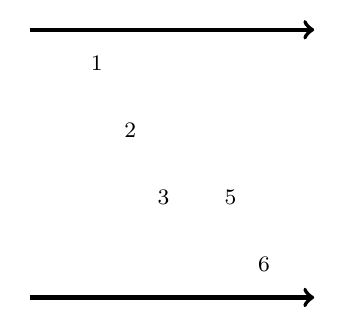
\begin{tikzpicture}[scale=0.85]
\draw[line width=1.5pt,->] (-0.5,3)--(3.75,3);
    \sq{0}{3};   \node at (0.5,2.5) {\footnotesize $1$};
    \sq{0.5}{2}; \node at (1,1.5)   {\footnotesize $2$};
    \sq{1}{1};   \node at (1.5,0.5) {\footnotesize $3$};
    \sq{2}{1};   \node at (2.5,0.5) {\footnotesize $5$};
    \sq{2.5}{0}; \node at (3,-0.5)  {\footnotesize $6$};
\draw[line width=1.5pt,->] (-0.5,-1)--(3.75,-1);
\end{tikzpicture}
\end{tabular}
\caption{}\label{fig:permexheap0.1}
\end{subfigure}
\begin{subfigure}{0.3\textwidth} \centering
\begin{tabular}{cc}
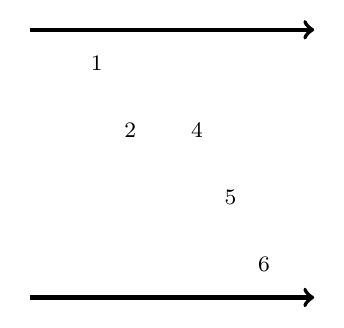
\begin{tikzpicture}[scale=0.85]
\draw[line width=1.5pt,->] (-0.5,3)--(3.75,3);
    \sq{0}{3};   \node at (0.5,2.5) {\footnotesize $1$};
    \sq{0.5}{2}; \node at (1,1.5)   {\footnotesize $2$};
    \sq{1.5}{2}; \node at (2,1.5)   {\footnotesize $4$};
    \sq{2}{1};   \node at (2.5,0.5) {\footnotesize $5$};
    \sq{2.5}{0}; \node at (3,-0.5)  {\footnotesize $6$};
\draw[line width=1.5pt,->] (-0.5,-1)--(3.75,-1);
\end{tikzpicture}
\end{tabular}
\caption{}\label{fig:permexheap0.2}
\end{subfigure}
\caption{The cylindrical heaps for Example~\ref{ex:swap}.}
\end{figure} \end{center}
    
    We claim that $w$ and $y$ are conjugate.
    Let $x$ have reduced expression \begin{equation} \x = 345623451234 = (3456)(2345)(1234). \end{equation}
    Then the heap $H({\x}{\w}{\x^{-1}})$ is shown in Figure~\ref{fig:permexheap1.1}. 
    By applying Lemma~\ref{lem:boomerang} to $\textcolor{blue}{123} \textcolor{ggreen}{4321}$, denoted in $H({\x}{\w}{\x^{-1}})$ by hatched blocks, we obtain the heap in Figure~\ref{fig:permexheap1.2}.
    Now, we apply Lemma~\ref{lem:stst} to the extra long $54$-chain in the heap in Figure~\ref{fig:permexheap1.2}, denoted by hatched blocks.
    Then, we have an extra long $43$-chain to which we can apply Lemma~\ref{lem:stst}. Continuing in this manner, we get the heap shown in Figure~\ref{fig:permexheap2}.
    
    We can apply Lemma~\ref{lem:boomerang} to $\textcolor{ggreen}{2345432}$ (hatched) to get the heap shown in Figure~\ref{fig:permexheap3}.
    Now we apply Lemma~\ref{lem:stst} to the extra long $65$-chain (hatched). Then, we have an extra long $54$-chain to which we can apply Lemma~\ref{lem:stst}.
    Continuing, we apply Lemma~\ref{lem:stst} to the extra long $43$-chain and the extra long $32$-chain and we get the heap shown in Figure~\ref{fig:permexheap4}.
    Finally, we apply Lemma~\ref{lem:boomerang} to $\textcolor{ggreen}{3456543}$ (hatched) and get the heap shown in Figure~\ref{fig:permexheap5}.
    We can cancel the adjacent 6 blocks (checked), followed by adjacent 5 blocks, adjacent 4 blocks, and adjacent 3 blocks. After all the cancellation, we get the heap shown in Figure~\ref{fig:permexheap6}, which yields the desired result.
\end{example}

\begin{figure}[htpb] \centering
\begin{subfigure}{0.3\textwidth} \centering \vspace{162pt}
\begin{tikzpicture}[scale=0.95]
    \sqor{1}{12};    \node at (1.5,11.5) {\footnotesize $3$};
    \sqor{0.5}{11};  \node at (1,10.5)   {\footnotesize $2$};
    \sqor{1.5}{11};  \node at (2,10.5)   {\footnotesize $4$};
    \sqor{0}{10};    \node at (0.5,9.5)  {\footnotesize $1$};
    \sqor{1}{10};    \node at (1.5,9.5)  {\footnotesize $3$};
    \sqor{2}{10};    \node at (2.5,9.5)  {\footnotesize $5$};
    \sqor{0.5}{9};   \node at (1,8.5)    {\footnotesize $2$};
    \sqor{1.5}{9};   \node at (2,8.5)    {\footnotesize $4$};
    \sqor{2.5}{9};   \node at (3,8.5)    {\footnotesize $6$};
    \sqblhash{0}{8}; \node at (0.5,7.5)  {\footnotesize $1$};
    \sqor{1}{8};     \node at (1.5,7.5)  {\footnotesize $3$};
    \sqor{2}{8};     \node at (2.5,7.5)  {\footnotesize $5$};
    \sqblhash{0.5}{7};\node at (1,6.5)   {\footnotesize $2$};
    \sqor{1.5}{7};   \node at (2,6.5)    {\footnotesize $4$};
    \sqblhash{1}{6}; \node at (1.5,5.5)  {\footnotesize $3$};
    \sqbl{2}{6};     \node at (2.5,5.5)  {\footnotesize $5$};
    \sqgrhash{1.5}{5};\node at (2,4.5)   {\footnotesize $4$};
    \sqbl{2.5}{5};   \node at (3,4.5)    {\footnotesize $6$};
    \sqgrhash{1}{4}; \node at (1.5,3.5)  {\footnotesize $3$};
    \sqgr{2}{4};     \node at (2.5,3.5)  {\footnotesize $5$};
    \sqgrhash{0.5}{3};\node at (1,2.5)   {\footnotesize $2$};
    \sqgr{1.5}{3};   \node at (2,2.5)    {\footnotesize $4$};
    \sqgr{2.5}{3};   \node at (3,2.5)    {\footnotesize $6$};
    \sqgrhash{0}{2}; \node at (0.5,1.5)  {\footnotesize $1$};
    \sqgr{1}{2};     \node at (1.5,1.5)  {\footnotesize $3$};
    \sqgr{2}{2};     \node at (2.5,1.5)  {\footnotesize $5$};
    \sqgr{0.5}{1};   \node at (1,0.5)    {\footnotesize $2$};
    \sqgr{1.5}{1};   \node at (2,0.5)    {\footnotesize $4$};
    \sqgr{1}{0};     \node at (1.5,-0.5) {\footnotesize $3$};
\end{tikzpicture}
\caption{}\label{fig:permexheap1.1}
\end{subfigure}
\begin{subfigure}{0.3\textwidth} \centering
\begin{tikzpicture}[scale=0.95]
    \sqor{1}{12};    \node at (1.5,11.5) {\footnotesize $3$};
    \sqor{0.5}{11};  \node at (1,10.5)   {\footnotesize $2$};
    \sqor{1.5}{11};  \node at (2,10.5)   {\footnotesize $4$};
    \sqor{0}{10};    \node at (0.5,9.5)  {\footnotesize $1$};
    \sqor{1}{10};    \node at (1.5,9.5)  {\footnotesize $3$};
    \sqor{2}{10};    \node at (2.5,9.5)  {\footnotesize $5$};
    \sqor{0.5}{9};   \node at (1,8.5)    {\footnotesize $2$};
    \sqor{1.5}{9};   \node at (2,8.5)    {\footnotesize $4$};
    \sqor{2.5}{9};   \node at (3,8.5)    {\footnotesize $6$};
    \sqor{1}{8};     \node at (1.5,7.5)  {\footnotesize $3$};
    \sqorhash{2}{8}; \node at (2.5,7.5)  {\footnotesize $5$};
    \sqorhash{1.5}{7};\node at (2,6.5)   {\footnotesize $4$};
    \sqblhash{2}{6}; \node at (2.5,5.5)  {\footnotesize $5$};
    \sqgrhash{1.5}{5};\node at (2,4.5)   {\footnotesize $4$};
    \sqbl{1}{4};     \node at (1.5,3.5)  {\footnotesize $3$};
    \sqbl{0.5}{3};   \node at (1,2.5)    {\footnotesize $2$};
    \sqbl{0}{2};     \node at (0.5,1.5)  {\footnotesize $1$};
    \sqgr{0.5}{1};   \node at (1,0.5)    {\footnotesize $2$};
    \sqgr{1}{0};     \node at (1.5,-0.5) {\footnotesize $3$};
    \sqgr{1.5}{-1};  \node at (2,-1.5)   {\footnotesize $4$};
    \sqbl{2.5}{-1};  \node at (3,-1.5)   {\footnotesize $6$};
    \sqgr{2}{-2};    \node at (2.5,-2.5) {\footnotesize $5$};
    \sqgr{1.5}{-3};  \node at (2,-3.5)   {\footnotesize $4$};
    \sqgr{2.5}{-3};  \node at (3,-3.5)   {\footnotesize $6$};
    \sqgr{1}{-4};    \node at (1.5,-4.5) {\footnotesize $3$};
    \sqgr{2}{-4};    \node at (2.5,-4.5) {\footnotesize $5$};
    \sqgr{0.5}{-5};  \node at (1,-5.5)   {\footnotesize $2$};
    \sqgr{1.5}{-5};  \node at (2,-5.5)   {\footnotesize $4$};
    \sqgr{1}{-6};    \node at (1.5,-6.5) {\footnotesize $3$};
\end{tikzpicture}
\caption{}\label{fig:permexheap1.2}
\end{subfigure}
\begin{subfigure}{0.3\textwidth} \centering \vspace{214pt}
\begin{tikzpicture}[scale=0.95]
    \sqor{1}{12};    \node at (1.5,11.5) {\footnotesize $3$};
    \sqor{1.5}{11};  \node at (2,10.5)   {\footnotesize $4$};
    \sqor{0}{12};    \node at (0.5,11.5) {\footnotesize $1$};
    \sqor{2}{10};    \node at (2.5,9.5)  {\footnotesize $5$};
    \sqor{0.5}{11};  \node at (1,10.5)   {\footnotesize $2$};
    \sqor{2.5}{9};   \node at (3,8.5)    {\footnotesize $6$};
    \sqor{1}{10};    \node at (1.5,9.5)  {\footnotesize $3$};
    \sqor{1.5}{9};   \node at (2,8.5)    {\footnotesize $4$};
    \sqbl{2}{8};     \node at (2.5,7.5)  {\footnotesize $5$};
    
    \sqgrhash{0.5}{9};   \node at (1,8.5)    {\footnotesize $2$};
    \sqgrhash{1}{8};     \node at (1.5,7.5)  {\footnotesize $3$};
    \sqgrhash{1.5}{7};   \node at (2,6.5)    {\footnotesize $4$};
    \sqbl{2.5}{7};       \node at (3,6.5)    {\footnotesize $6$};
    \sqgrhash{2}{6};     \node at (2.5,5.5)  {\footnotesize $5$};
    \sqgrhash{1.5}{5};   \node at (2,4.5)    {\footnotesize $4$};
    \sqgrhash{2.5}{5};   \node at (3,4.5)    {\footnotesize $6$};
    \sqgrhash{1}{4};     \node at (1.5,3.5)  {\footnotesize $3$};
    \sqgr{2}{4};         \node at (2.5,3.5)  {\footnotesize $5$};
    \sqgrhash{0.5}{3};   \node at (1,2.5)    {\footnotesize $2$};
    \sqgr{1.5}{3};       \node at (2,2.5)    {\footnotesize $4$};
    \sqgr{1}{2};         \node at (1.5,1.5)  {\footnotesize $3$};
\end{tikzpicture}
\caption{}\label{fig:permexheap2}
\end{subfigure}
\caption{The heaps for Example~\ref{ex:swap}.}\label{}
\end{figure}
\begin{figure}[H] \centering
\ContinuedFloat
\begin{subfigure}{0.3\textwidth} \centering \vspace{-46pt}
\begin{tikzpicture}[scale=0.925]
    \sqor{1}{12};     \node at (1.5,11.5) {\footnotesize $3$};
    \sqor{1.5}{11};   \node at (2,10.5)   {\footnotesize $4$};
    \sqor{0}{12};     \node at (0.5,11.5) {\footnotesize $1$};
    \sqor{2}{10};     \node at (2.5,9.5)  {\footnotesize $5$};
    \sqor{0.5}{11};   \node at (1,10.5)   {\footnotesize $2$};
    \sqorhash{2.5}{9};\node at (3,8.5)    {\footnotesize $6$};
    \sqor{1}{10};     \node at (1.5,9.5)  {\footnotesize $3$};
    \sqor{1.5}{9};    \node at (2,8.5)    {\footnotesize $4$};
    \sqblhash{2}{8};  \node at (2.5,7.5)  {\footnotesize $5$};
    
    \sqgr{0.5}{3};    \node at (1,2.5)    {\footnotesize $2$};
    \sqgr{1}{4};      \node at (1.5,3.5)  {\footnotesize $3$};
    \sqgr{1.5}{5};    \node at (2,4.5)    {\footnotesize $4$};
    \sqgrhash{2}{6};  \node at (2.5,5.5)  {\footnotesize $5$};
    \sqblhash{2.5}{7};\node at (3,6.5)    {\footnotesize $6$};
    \sqgr{1}{2};      \node at (1.5,1.5)  {\footnotesize $3$};
    \sqgr{1.5}{1};    \node at (2,0.5)    {\footnotesize $4$};
    \sqgr{2}{0};      \node at (2.5,-0.5) {\footnotesize $5$};
    \sqgr{2.5}{-1};   \node at (3,-1.5)   {\footnotesize $6$};
    \sqgr{1.5}{-1};   \node at (2,-1.5)   {\footnotesize $4$};
    \sqgr{1}{-2};     \node at (1.5,-2.5) {\footnotesize $3$};
    \sqgr{2}{-2};     \node at (2.5,-2.5) {\footnotesize $5$};
    \sqgr{0.5}{-3};   \node at (1,-3.5)   {\footnotesize $2$};
    \sqgr{1.5}{-3};   \node at (2,-3.5)   {\footnotesize $4$};
    \sqgr{1}{-4};     \node at (1.5,-4.5) {\footnotesize $3$};
\end{tikzpicture}
\caption{}\label{fig:permexheap3}
\end{subfigure}
\begin{subfigure}{0.3\textwidth} \centering \vspace{108pt}
\begin{tikzpicture}[scale=0.95]
    \sqor{0}{10};       \node at (0.5,9.5)  {\footnotesize $1$};
    \sqor{0.5}{9};      \node at (1,8.5)    {\footnotesize $2$};
    \sqor{1}{8};        \node at (1.5,7.5)  {\footnotesize $3$};
    \sqor{1.5}{7};      \node at (2,6.5)    {\footnotesize $4$};
    \sqbl{2}{6};        \node at (2.5,5.5)  {\footnotesize $5$};
    \sqbl{2.5}{5};      \node at (3,4.5)    {\footnotesize $6$};
    \sqgrhash{1}{6};    \node at (1.5,5.5)  {\footnotesize $3$};
    \sqgrhash{1.5}{5};  \node at (2,4.5)    {\footnotesize $4$};
    \sqgrhash{2}{4};    \node at (2.5,3.5)  {\footnotesize $5$};
    \sqgrhash{2.5}{3};  \node at (3,2.5)    {\footnotesize $6$};
    \sqgrhash{2}{2};    \node at (2.5,1.5)  {\footnotesize $5$};
    \sqgrhash{1.5}{1};  \node at (2,0.5)    {\footnotesize $4$};
    \sqgrhash{1}{0};    \node at (1.5,-0.5) {\footnotesize $3$};
\end{tikzpicture}
\caption{}\label{fig:permexheap4}
\end{subfigure}
\begin{subfigure}{0.3\textwidth} \centering \vspace{50pt}
\begin{tikzpicture}[scale=0.95]
    \sqor{0}{10};       \node at (0.5,9.5)  {\footnotesize $1$};
    \sqor{0.5}{9};      \node at (1,8.5)    {\footnotesize $2$};
    \sqor{1}{8};        \node at (1.5,7.5)  {\footnotesize $3$};
    \sqor{1.5}{7};      \node at (2,6.5)    {\footnotesize $4$};
    \sqbl{2}{6};        \node at (2.5,5.5)  {\footnotesize $5$};
    \sqblcheck{2.5}{5}; \node at (3,4.5)    {\footnotesize $6$};
    \sqgr{1}{1};        \node at (1.5,0.5)  {\footnotesize $3$};
    \sqgr{1.5}{2};      \node at (2,1.5)    {\footnotesize $4$};
    \sqgr{2}{3};        \node at (2.5,2.5)  {\footnotesize $5$};
    \sqgrcheck{2.5}{4}; \node at (3,3.5)    {\footnotesize $6$};
    \sqgr{2}{-1};       \node at (2.5,-1.5) {\footnotesize $5$};
    \sqgr{1.5}{0};      \node at (2,-0.5)   {\footnotesize $4$};
    \sqgr{2.5}{-2};     \node at (3,-2.5)   {\footnotesize $6$};
\end{tikzpicture}
\caption{}\label{fig:permexheap5}
\end{subfigure}
\begin{subfigure}{\textwidth} \centering \vspace{10pt}
\begin{tikzpicture}[scale=0.95]
    \sqor{0}{6};       \node at (0.5,5.5)  {\footnotesize $1$};
    \sqor{0.5}{5};     \node at (1,4.5)    {\footnotesize $2$};
    \sqgr{1.5}{5};     \node at (2,4.5)    {\footnotesize $4$};
    \sqgr{2}{4};       \node at (2.5,3.5)  {\footnotesize $5$};
    \sqgr{2.5}{3};     \node at (3,2.5)    {\footnotesize $6$};
\end{tikzpicture}
\caption{}\label{fig:permexheap6}
\end{subfigure}
\caption{The heaps for Example~\ref{ex:swap} (continued).}\label{fig:permexheaps}
\end{figure}


    We can generalize the technique used in the previous example to prove the following lemma, which allows us to permute two adjacent diagonal chunks.

\begin{lemma}\label{lem:swap}
Let $w,y \in \CFC(A_n)$ such that $H(w)$ and $H(y)$ are simple, each consisting of two chunks as in Figure~\ref{fig:swap1}, where the chunk starting at 1 has size $k$ and the adjacent chunk has size $m$ and $k'=k+m$. Then $w$ and $y$ are conjugate.
\end{lemma}

\begin{center} \begin{figure}[H] \centering
\begin{subfigure}{0.45\textwidth} \centering
\begin{tabular}{@{}c@{}c}
\begin{tikzpicture}
    \sq{0}{3};    \node at (0.5,2.5)   {\scalebox{0.8}{$1$}};
    \sq{0.5}{2};  \node at (1,1.5)     {\scalebox{0.8}{$2$}};
                  \node at (1.5,0.7)   {$\ddots$};
    \sq{1.5}{0};  \node at (2,-0.5)    {\scalebox{0.8}{$k$}};
\end{tikzpicture} &
\begin{tikzpicture}
    \sq{2.5}{3};  \node at (3,2.5)     {\scalebox{0.8}{$k+2$}};
    \sq{3}{2};    \node at (3.5,1.5)   {\scalebox{0.8}{$k+3$}};
                  \node at (4,0.7)     {$\ddots$};
    \sq{4}{0};    \node at (4.5,-0.5)  {\scalebox{0.8}{$k'+1$}};
\end{tikzpicture}
\end{tabular}
\caption{}\label{fig:swap1}
\end{subfigure}
\begin{subfigure}{0.45\textwidth} \centering
\begin{tabular}{@{}c@{}c} \centering
\begin{tikzpicture}
    \sq{0}{3};    \node at (0.5,2.5) {\scalebox{0.8}{$1$}};
    \sq{0.5}{2};  \node at (1,1.5)   {\scalebox{0.8}{$2$}};
                  \node at (1.5,0.7) {$\ddots$};
    \sq{1.5}{0};  \node at (2,-0.5)  {\scalebox{0.8}{$m$}};
\end{tikzpicture} &
\begin{tikzpicture}
    \sq{2.5}{3};  \node at (3,2.5)   {\scalebox{0.8}{$m+2$}};
    \sq{3}{2};    \node at (3.5,1.5) {\scalebox{0.8}{$m+3$}};
                  \node at (4,0.7)   {$\ddots$};
    \sq{4}{0};    \node at (4.5,-0.5){\scalebox{0.8}{$k'+1$}};
\end{tikzpicture} \end{tabular}
\caption{}\label{fig:swap2}
\end{subfigure}
\caption{The heaps for Lemma~\ref{lem:swap}.}\label{}
\end{figure} \end{center}

\begin{proof} We first consider the case $k>m$.
    Let $x \in W(A_n)$ have a reduced expression $\x$ that consists of $m+1$ ascending subwords of $k+1$ generators each, starting with $(m+1)(m+2) \cdots (k'+1)$ and being such that the sequence of first generators of each subword descends to 1 (as in Example~\ref{ex:swap}).
    That is, $$\x = \underbrace{(m+1)(m+2) \cdots (k'+1)}_{1} \underbrace{(m)(m+1) \cdots (k')}_{2} \cdots \underbrace{(2)(3) \cdots (k)}_{m} \underbrace{(1)(2) \cdots (k+1)}_{m+1}.$$
    Conjugate $w$ by $x$, and consider the heap $H({\x}{\w}{\x^{-1}})$, shown in Figure~\ref{fig:permheap1}, where $k'=k+m$ and \textcolor{orange}{orange} blocks correspond to the heap of $\x$, \textcolor{blue}{blue} blocks correspond to the heap of $w$, and \textcolor{ggreen}{green} blocks correspond to the heap of $\x^{-1}$.
    Now, to the heap in Figure~\ref{fig:permheap1}, we apply Lemma~\ref{lem:boomerang} to $$\textcolor{blue}{(1)(2) \cdots (k)} \textcolor{ggreen}{(k+1)(k) \cdots (2)(1)},$$ denoted by hatched blocks, to get the heap shown in Figure~\ref{fig:permheap2}.
    
    Then, as in the proof of Lemma~\ref{lem:slide}, apply Lemma~\ref{lem:stst} to the extra long $(k+2)(k+1)$-chain, denoted in the heap in Figure~\ref{fig:permheap2} as hatched blocks.
    This creates an extra long $(k+1)(k)$-chain.
    Continuing this process $k$ times, we get the heap shown in Figure~\ref{fig:permheap3} since the \textcolor{blue}{blue} $(1)(2)\cdots(k)(k+2)$, \textcolor{ggreen}{green} $(k+1)$, and \textcolor{orange}{orange} $(2)(3) \cdots (k+2)$ blocks in Figure~\ref{fig:permheap2} cancel via the iterations of Lemma~\ref{lem:stst} with extra long $s_is_j$-chains.
    
    Then, after $m$ steps as above, we get the heap shown in Figure~\ref{fig:permheap4}.
    Finally, we apply Lemma~\ref{lem:boomerang} to the blocks labeled $$\textcolor{ggreen}{(m+1)(m+2) \cdots (k')(k'+1)(k') \cdots (m+2)(m+1)},$$ denoted in the heap in Figure~\ref{fig:permheap4} by hatched blocks, to get the heap shown in Figure~\ref{fig:permheap5}.
    There are adjacent $k'+1$ blocks that cancel, denoted in the heap by checked blocks, followed by adjacent $k'$ blocks, and so on. After the cancellation, we get the heap shown in Figure~\ref{fig:permheap6} and the result follows.
    
    In the case where $k<m$, conjugate $w$ by $x^{-1}$, as given above, to obtain $y$.
\end{proof}

\begin{remark}\label{rem:permute} If the heap of $w$ is not simple, we can perform a sequence of cyclic shifts and applications of Lemma~\ref{lem:slide} and Remark~\ref{rem:slide} to obtain a simple heap, and, after applying Lemma~\ref{lem:swap}, we can reverse the cyclic shifts and applications of Lemma~\ref{lem:slide} and Remark~\ref{rem:slide}.
\end{remark}

\begin{center} \begin{figure}[htpb] \centering
\begin{tabular}{cc}
\begin{subfigure}{0.45\textwidth} \centering \vspace{124pt}
\begin{tikzpicture}[scale=0.82]
    \sqblhash{0}{9};   \node at (0.5,8.5)   {\scalebox{0.75}{$1$}};
    \sqblhash{0.5}{8}; \node at (1,7.5)     {\scalebox{0.75}{$2$}};
                       \node at (1.8,6.6)   {$\ddots$};
    \sqblhash{2}{6};   \node at (2.5,5.5)   {\scalebox{0.75}{$k$}};
    \sqbl{3}{6};       \node at (3.5,5.5)   {\scalebox{0.75}{$k+2$}};
    \sqbl{3.5}{5};     \node at (4,4.5)     {\scalebox{0.75}{$k+3$}};
                       \node at (4.8,3.65)  {$\ddots$};
    \sqbl{5}{3};       \node at (5.5,2.5)   {\scalebox{0.75}{$k'$}};
    \sqbl{5.5}{2};     \node at (6,1.5)     {\scalebox{0.75}{$k'+1$}};

    \sqor{2.5}{7};     \node at (3,6.5)     {\scalebox{0.75}{$k+1$}};
                       \node at (2.25,7.6)  {$\ddots$};
    \sqor{1}{9};       \node at (1.5,8.5)   {\scalebox{0.75}{$3$}};
    \sqor{0.5}{10};    \node at (1,9.5)     {\scalebox{0.75}{$2$}};
    \sqor{0}{11};      \node at (0.5,10.5)  {\scalebox{0.75}{$1$}};
    \sqor{3}{8};       \node at (3.5,7.5)   {\scalebox{0.75}{$k+2$}};
                       \node at (2.75,8.6)  {$\ddots$};
    \sqor{1.5}{10};    \node at (2,9.5)     {\scalebox{0.75}{$4$}};
    \sqor{1}{11};      \node at (1.5,10.5)  {\scalebox{0.75}{$3$}};
    \sqor{0.5}{12};    \node at (1,11.5)    {\scalebox{0.75}{$2$}};
                       \node at (2,12.5)    {$\iddots$};
                       \node at (4.5,8.5)   {$\iddots$};
                       \node at (3,11.5)    {$\iddots$};
                       \node at (5.1,11.6)  {$\ddots$};
                       \node at (4,10.5)    {$\cdots$};
                       \node at (4,9.5)     {$\cdots$};
    \sqor{3}{14};      \node at (3.5,13.5)  {\scalebox{0.75}{$m+1$}};
    \sqor{3.5}{13};    \node at (4,12.5)    {\scalebox{0.75}{$m+2$}};
    \sqor{5.5}{11};    \node at (6,10.5)    {\scalebox{0.75}{$k'+1$}};
    \sqor{5}{10};      \node at (5.5,9.5)   {\scalebox{0.75}{$k'$}};
    
    \sqgrhash{2.5}{5}; \node at (3,4.5)     {\scalebox{0.75}{$k+1$}};
    \sqgrhash{2}{4};   \node at (2.5,3.5)   {\scalebox{0.75}{$k$}};
    \sqgr{3}{4};       \node at (3.5,3.5)   {\scalebox{0.75}{$k+2$}};
                   
    \sqgr{4.5}{2};     \node at (5,1.5)     {\scalebox{0.75}{$k'-1$}};
    \sqgr{5}{1};       \node at (5.5,0.5)   {\scalebox{0.75}{$k'$}};
    \sqgr{5.5}{0};     \node at (6,-0.5)    {\scalebox{0.75}{$k'+1$}};
                       \node at (5,-1.5)    {$\iddots$};
    \sqgrhash{0.5}{2}; \node at (1,1.5)     {\scalebox{0.75}{$2$}};
    \sqgrhash{0}{1};   \node at (0.5,0.5)   {\scalebox{0.75}{$1$}};
    \sqgr{1}{1};       \node at (1.5,0.5)   {\scalebox{0.75}{$3$}};
    \sqgr{0.5}{0};     \node at (1,-0.5)    {\scalebox{0.75}{$2$}};
    \sqgr{1.5}{2};     \node at (2,1.5)     {\scalebox{0.75}{$4$}};
                       \node at (2,-1.5)    {$\ddots$};
    \sqgr{3}{-3};      \node at (3.5,-3.5)  {\scalebox{0.75}{$m+1$}};
    \sqgr{2.5}{-2};    \node at (3,-2.5)    {\scalebox{0.75}{$m$}};
    \sqgr{3.5}{-2};    \node at (4,-2.5)    {\scalebox{0.75}{$m+2$}};
                       \node at (1.8,2.5)   {$\iddots$};
                       \node at (2.8,2.5)   {$\iddots$};
                       \node at (3.5,1.5)   {$\cdots$};
                       \node at (3.5,0.5)   {$\cdots$};
                       \node at (3.5,-0.5)  {$\cdots$};
                       \node at (4.3,2.5)   {$\ddots$};
\end{tikzpicture}
\caption{}\label{fig:permheap1}
\end{subfigure} &
\begin{subfigure}{0.45\textwidth} \centering \vspace{-45pt}
\begin{tikzpicture}[scale=0.8]
    \sqbl{0}{5};        \node at (0.5,4.5)   {\scalebox{0.7}{$1$}};
    \sqbl{0.5}{6};      \node at (1,5.5)     {\scalebox{0.7}{$2$}};
    \sqbl{2}{8};        \node at (2.5,7.5)   {\scalebox{0.7}{$k$}};
    \sqblhash{3}{10};   \node at (3.5,9.5)   {\scalebox{0.7}{$k+2$}};
    \sqbl{3.5}{1};      \node at (4,0.5)     {\scalebox{0.7}{$k+3$}};
    \sqbl{3}{0};        \node at (3.5,-0.5)  {\scalebox{0.7}{$k+2$}};
                        \node at (5.1,-0.35) {$\ddots$};
    \sqbl{5}{-1};       \node at (5.5,-1.5)  {\scalebox{0.7}{$k'$}};
    \sqbl{5.5}{-2};     \node at (6,-2.5)    {\scalebox{0.7}{$k'+1$}};

    \sqorhash{2.5}{11}; \node at (3,10.5)    {\scalebox{0.7}{$k+1$}};
                        \node at (2.25,11.6) {$\ddots$};
    \sqor{1}{13};       \node at (1.5,12.5)  {\scalebox{0.7}{$3$}};
    \sqor{0.5}{14};     \node at (1,13.5)    {\scalebox{0.7}{$2$}};
    \sqor{0}{15};       \node at (0.5,14.5)  {\scalebox{0.7}{$1$}};
    \sqorhash{3}{12};   \node at (3.5,11.5)  {\scalebox{0.7}{$k+2$}};
                        \node at (2.75,12.8) {$\ddots$};
    \sqor{1.5}{14};     \node at (2,13.5)    {\scalebox{0.7}{$4$}};
    \sqor{1}{15};       \node at (1.5,14.5)  {\scalebox{0.7}{$3$}};
    \sqor{0.5}{16};     \node at (1,15.5)    {\scalebox{0.7}{$2$}};
                        \node at (2,16.5)    {$\iddots$};
                        \node at (4.5,12.5)  {$\iddots$};
                        \node at (2.75,16)   {$\iddots$};
                        \node at (5.1,15.6)  {$\ddots$};
                        \node at (4,14.5)    {$\cdots$};
                        \node at (4,13.5)    {$\cdots$};
    \sqor{3}{18};       \node at (3.5,17.5)  {\scalebox{0.7}{$m+1$}};
    \sqor{3.5}{17};     \node at (4,16.5)    {\scalebox{0.7}{$m+2$}};
    \sqor{5.5}{15};     \node at (6,14.5)    {\scalebox{0.7}{$k'+1$}};
    \sqor{5}{14};       \node at (5.5,13.5)  {\scalebox{0.7}{$k'$}};
                    
    \sqgrhash{2.5}{9};  \node at (3,8.5)     {\scalebox{0.7}{$k+1$}};
    \sqgr{2.5}{1};      \node at (3,0.5)     {\scalebox{0.7}{$k+1$}};
    \sqgr{2}{2};        \node at (2.5,1.5)   {\scalebox{0.7}{$k$}};
                        \node at (1.75,6.6)  {$\iddots$};
                        \node at (1.75,2.5)  {$\ddots$};
    \sqgr{3}{0};        \node at (3.5,-0.5)  {\scalebox{0.7}{$k+2$}};
    \sqgr{4.5}{-4};     \node at (5,-4.5)    {\scalebox{0.7}{$k'-1$}};
    \sqgr{5}{-3};       \node at (5.5,-3.5)  {\scalebox{0.7}{$k'$}};
    \sqgr{4.5}{-2};     \node at (5,-2.5)    {\scalebox{0.7}{$k'-1$}};
    \sqgr{5.5}{-4};     \node at (6,-4.5)    {\scalebox{0.7}{$k'+1$}};
                        \node at (5,-5.5)    {$\iddots$};
    \sqgr{0.5}{4};      \node at (1,3.5)     {\scalebox{0.7}{$2$}};
    \sqgr{1}{-3};       \node at (1.5,-3.5)  {\scalebox{0.7}{$3$}};
    \sqgr{0.5}{-4};     \node at (1,-4.5)    {\scalebox{0.7}{$2$}};
    \sqgr{1.5}{-2};     \node at (2,-2.5)    {\scalebox{0.7}{$4$}};
                        \node at (2,-5.5)    {$\ddots$};
    \sqgr{3}{-7};       \node at (3.5,-7.5)  {\scalebox{0.7}{$m+1$}};
    \sqgr{2.5}{-6};     \node at (3,-6.5)    {\scalebox{0.7}{$m$}};
    \sqgr{3.5}{-6};     \node at (4,-6.5)    {\scalebox{0.7}{$m+2$}};
                        \node at (2.7,-1.4)  {$\iddots$};
                        \node at (3.5,-2.5)  {$\cdots$};
                        \node at (3.5,-3.5)  {$\cdots$};
                        \node at (3.5,-4.5)  {$\cdots$};
                        \node at (4.4,-1.4)  {$\ddots$};
\end{tikzpicture}
\caption{}\label{fig:permheap2}
\end{subfigure}
\end{tabular}
\caption{The heaps for Lemma~\ref{lem:swap}.}\label{}
\end{figure}
\begin{figure}[H] \centering
\ContinuedFloat
\begin{tabular}{cc}
\begin{subfigure}{0.45\textwidth} \centering
\begin{tikzpicture}
    \sqbl{0}{13};   \node at (0.5,12.5)  {\scalebox{0.85}{$1$}};
                    \node at (5,3.5)     {$\iddots$};
    \sqgr{0.5}{12}; \node at (1,11.5)    {\scalebox{0.85}{$2$}};
    
    \sqbl{3}{10};   \node at (3.5,9.5)   {\scalebox{0.85}{$k+2$}};
    \sqbl{3.5}{9};  \node at (4,8.5)     {\scalebox{0.85}{$k+3$}};
                    \node at (4.8,7.65)  {$\ddots$};
    \sqbl{5}{7};    \node at (5.5,6.5)   {\scalebox{0.85}{$k'$}};
    \sqbl{5.5}{6};  \node at (6,5.5)     {\scalebox{0.85}{$k'+1$}};

    \sqor{2.5}{11}; \node at (3,10.5)    {\scalebox{0.85}{$k+1$}};
    \sqor{3}{12};   \node at (3.5,11.5)  {\scalebox{0.85}{$k+2$}};
                    \node at (2.25,11.6) {$\ddots$};
                    \node at (3,12.7) {$\ddots$};
    \sqor{1}{13};   \node at (1.5,12.5)  {\scalebox{0.85}{$3$}};
    \sqor{0.5}{14}; \node at (1,13.5)    {\scalebox{0.85}{$2$}};
    \sqor{0}{15};   \node at (0.5,14.5)  {\scalebox{0.85}{$1$}};
    \sqor{1}{15};   \node at (1.5,14.5)  {\scalebox{0.85}{$3$}};
    \sqor{1.5}{14}; \node at (2,13.5) {\scalebox{0.85}{$4$}};
                    \node at (4.7,12.6)  {$\iddots$};
                    \node at (2.3,15.6)  {$\iddots$};
                    \node at (3,14.8)    {$\iddots$};
                    \node at (5.2,14.8)  {$\ddots$};
                    \node at (4,13.5)  {$\cdots$};
    \sqor{3}{17};   \node at (3.5,16.5)  {\scalebox{0.85}{$m+1$}};
    \sqor{3.5}{16}; \node at (4,15.5)    {\scalebox{0.85}{$m+2$}};
    \sqor{5.5}{14}; \node at (6,13.5)    {\scalebox{0.85}{$k'+1$}};
    \sqgr{2.5}{9};  \node at (3,8.5)     {\scalebox{0.85}{$k+1$}};
    \sqgr{2}{10};   \node at (2.5,9.5)   {\scalebox{0.85}{$k$}};
                    \node at (1.75,10.5) {$\ddots$};
    \sqgr{3}{8};    \node at (3.5,7.5)   {\scalebox{0.85}{$k+2$}};
                    
    \sqgr{4.5}{4};  \node at (5,3.5)     {\scalebox{0.85}{$k'-1$}};
    \sqgr{5}{5};    \node at (5.5,4.5)   {\scalebox{0.85}{$k'$}};
    \sqgr{4.5}{6};  \node at (5,5.5)     {\scalebox{0.85}{$k'-1$}};
    \sqgr{5.5}{4};  \node at (6,3.5)     {\scalebox{0.85}{$k'+1$}};

    \sqgr{1}{5};    \node at (1.5,4.5)   {\scalebox{0.85}{$3$}};
    \sqgr{0.5}{4};  \node at (1,3.5)     {\scalebox{0.85}{$2$}};
    \sqgr{1.5}{6};  \node at (2,5.5)     {\scalebox{0.85}{$4$}};
                    \node at (2,2.5)     {$\ddots$};
                    \node at (5,2.5)     {$\iddots$};
    \sqgr{3}{1};    \node at (3.5,0.5)   {\scalebox{0.85}{$m+1$}};
    \sqgr{2.5}{2};  \node at (3,1.5)     {\scalebox{0.85}{$m$}};
    \sqgr{3.5}{2};  \node at (4,1.5)     {\scalebox{0.85}{$m+2$}};
                    \node at (2.8,6.5)   {$\iddots$};
                    \node at (3.5,5.5)   {$\cdots$};
                    \node at (3.5,4.5)   {$\cdots$};
                    \node at (3.5,3.5)   {$\cdots$};
                    \node at (4.3,6.5)   {$\ddots$};
\end{tikzpicture}
\caption{}\label{fig:permheap3}
\end{subfigure} &
\begin{subfigure}{0.45\textwidth} \centering \vspace{30pt}
\begin{tikzpicture}
    \sqor{0}{13};   \node at (0.5,12.5)  {\scalebox{0.75}{$1$}};
    \sqor{0.5}{12}; \node at (1,11.5)    {\scalebox{0.75}{$2$}};
    \sqor{2.5}{9};  \node at (3,8.5)     {\scalebox{0.75}{$k+1$}};
    \sqor{2}{10};   \node at (2.5,9.5)   {\scalebox{0.75}{$k$}};
                    \node at (1.85,10.6) {$\ddots$};
    \sqbl{3}{8};    \node at (3.5,7.5)   {\scalebox{0.75}{$k+2$}};
                    \node at (4.25,6.75) {$\ddots$};
    \sqbl{5}{5};    \node at (5.5,4.5)   {\scalebox{0.75}{$k'$}};
    \sqbl{4.5}{6};  \node at (5,5.5)     {\scalebox{0.75}{$k'-1$}};
    \sqbl{5.5}{4};  \node at (6,3.5)     {\scalebox{0.75}{$k'+1$}};
    \sqgrhash{3}{6};    \node at (3.5,5.5)   {\scalebox{0.75}{$m+2$}};
    \sqgrhash{2.5}{7};  \node at (3,6.5)     {\scalebox{0.75}{$m+1$}};
                    \node at (4.25,4.75) {$\ddots$};
    \sqgrhash{5}{3};    \node at (5.5,2.5)   {\scalebox{0.75}{$k'$}};
    \sqgrhash{4.5}{4};  \node at (5,3.5)     {\scalebox{0.75}{$k'-1$}};
    \sqgrhash{5.5}{2};  \node at (6,1.5)     {\scalebox{0.75}{$k'+1$}};
    \sqgrhash{5}{1};    \node at (5.5,0.5)   {\scalebox{0.75}{$k'$}};
                    \node at (4.75,-0.5) {$\iddots$};
    \sqgrhash{3.5}{-1}; \node at (4,-1.5)    {\scalebox{0.75}{$m+2$}};
    \sqgrhash{3}{-2};   \node at (3.5,-2.5)  {\scalebox{0.75}{$m+1$}};
\end{tikzpicture}
\caption{}\label{fig:permheap4}
\end{subfigure}
\end{tabular}
\caption{The heaps for Lemma~\ref{lem:swap} (continued).}\label{}
\end{figure}

\clearpage

\begin{figure}[H] \centering
\ContinuedFloat
\begin{tabular}{cc} \centering
\begin{subfigure}{0.5\textwidth} \centering
\begin{tikzpicture}
    \sqor{0}{13};   \node at (0.5,12.5)  {\scalebox{0.75}{$1$}};
    \sqor{0.5}{12}; \node at (1,11.5)    {\scalebox{0.75}{$2$}};
    \sqor{2.5}{9};  \node at (3,8.5)     {\scalebox{0.75}{$k+1$}};
    \sqor{2}{10};   \node at (2.5,9.5)   {\scalebox{0.75}{$k$}};
                    \node at (1.85,10.6) {$\ddots$};
    \sqbl{3}{8};    \node at (3.5,7.5)   {\scalebox{0.75}{$k+2$}};
                    \node at (4.4,6.6) {$\ddots$};
    \sqbl{5}{6};    \node at (5.5,5.5)   {\scalebox{0.75}{$k'$}};
    \sqblcheck{5.5}{5};  \node at (6,4.5) {\scalebox{0.75}{$k'+1$}};
    \sqgrcheck{5.5}{4};  \node at (6,3.5) {\scalebox{0.75}{$k'+1$}};
    \sqgr{3}{1};    \node at (3.5,0.5)    {\scalebox{0.75}{$m+2$}};
    \sqgr{2.5}{0};  \node at (3,-0.5)     {\scalebox{0.75}{$m+1$}};
                    \node at (4.4,1.7)    {$\iddots$};
    \sqgr{5}{3};    \node at (5.5,2.5)    {\scalebox{0.75}{$k'$}};
    \sqgr{5.5}{-4}; \node at (6,-4.5)     {\scalebox{0.75}{$k'+1$}};
    \sqgr{5}{-3};   \node at (5.5,-3.5)   {\scalebox{0.75}{$k'$}};
                    \node at (4.4,-2.5)   {$\ddots$};
    \sqgr{3}{-1};   \node at (3.5,-1.5)   {\scalebox{0.75}{$m+2$}};
\end{tikzpicture}
\caption{}\label{fig:permheap5}
\end{subfigure} &
\begin{subfigure}{0.5\textwidth} \centering \vspace{4.3in}
\begin{tikzpicture}
    \sqor{0}{3};    \node at (0.5,2.5)   {\scalebox{0.85}{$1$}};
    \sqor{0.5}{2};  \node at (1,1.5)     {\scalebox{0.85}{$2$}};
                    \node at (1.5,0.7)   {$\ddots$};
    \sqor{1.5}{0};  \node at (2,-0.5)    {\scalebox{0.85}{$m$}};
    \sqgr{2.5}{0};  \node at (3,-0.5)    {\scalebox{0.85}{$m+2$}};
    \sqgr{3}{-1};   \node at (3.5,-1.5)  {\scalebox{0.85}{$m+3$}};
                    \node at (4.25,-2.25){$\ddots$};
    \sqgr{4}{-3};   \node at (4.5,-3.5)  {\scalebox{0.85}{$k'+1$}};
\end{tikzpicture}
\caption{}\label{fig:permheap6}
\end{subfigure}
\end{tabular}
\caption{The heaps for Lemma~\ref{lem:swap} (continued).}
\end{figure} \end{center}

    We are now ready to prove Theorem~\ref{thm:conjiffring}.

\begin{proof}[Proof of Theorem~\ref{thm:conjiffring}] Suppose $w,y \in \CFC(A_n)$ are conjugate.
    Note that every chunk of size $\ell$ in $W(A_n)$ corresponds to a cycle of length $\ell+1$ with connected support in $S_{n+1}$.
    In particular, the chunk that corresponds to the group element $(k)(k+1) \cdots (k+m)$ corresponds to the $(m+2)$-cycle $(k~k+1~ \cdots ~ k+m~k+m+1)$.
    By assumption, as permutations, $w$ and $y$ in $S_{n+1}$ have the same cycle type. Suppose $w$ and $y$ each consist of products of disjoint cycles of lengths $k_{1}, k_{2}, \ldots, k_{s}$. In this case, it is not possible for $H(w)$ and $H(y)$ to have a different number of chunks. Furthermore, there are $n$ chunks of size $k$ in $H(w)$ if and only if there are $n$ chunks of size $k$ in $H(y)$. 
    Then both of $H(w)$ and $H(y)$ consist of chunks of sizes $k_{1}-1,k_{2}-1,\ldots,k_{s}-1$. That is, for every ring $R$ in $\hat{H}(w)$, there is a corresponding ring $R'$ in $\hat{H}(y)$. Then, we can permute and slide rings in $\hat{H}(w)$ as necessary to obtain $\hat{H}(y)$.
    Hence $\hat{H}(w)$ and $\hat{H}(y)$ are ring equivalent.

    Now, suppose $\hat{H}(w)$ and $\hat{H}(y)$ are ring equivalent. Then there exists some sequence of cyclic shifts, slides, and permutations of chunks that takes $\hat{H}(w)$ to $\hat{H}(y)$. We can perform these operations via conjugation, as in Lemmas~\ref{lem:slide} and~\ref{lem:swap} and Remarks~\ref{rem:slide} and~\ref{rem:permute}. Hence $w$ and $y$ are conjugate.
\end{proof}

    In the future, we hope to be able to generalize the notion of chunks and rings to CFC elements of Coxeter groups of types other than $A_n$ in order to have a result analogous to Theorem~\ref{thm:conjiffring}.
    We will need a different proof for an analogous theorem in Coxeter group of types other than $A_n$ since we used cycle type in the argument for the forward direction of the proof of Theorem~\ref{thm:conjiffring}.



